\vzmstitle{
	Геометрия множеств Стокса
}
\vzmsauthor{Артёмов}{Н.\,М.}
\vzmsinfo{Воронеж, ВГУ; \textit{nikitartemov@mail.ru} }
\vzmscaption

В изучении c помощью метода перевала~[1] асимптотики экспоненциальных интегралов,
зависящих от параметров, важную роль играют множества таких параметров,
при которых у фазовой функции имеются несколько критических точек с одинаковыми вещественными частями критических значений.
Такие множества получили название <<множества Стокса>>.
В случае типичных семейств, зависящих от параметров, их коразмерность равна единице.
Множества Стокса изучались в работах [2--4],
и были получены картинки объединения каустики и множеств Стокса в $\mathbb{R}^3$ для особенностей
$A_{4}, D_{4}^-, D_{4}^+, $ но при этом учитывались лишь компоненты (расширенного) множества Стокса,
соответствующие максимальным критическим значениям (поскольку лишь
\linebreak
они интересны с точки зрения изучения асимптотики экспоненциальных интегралов). В данном докладе мы опишем полные расширенные множества Стокса для особенностей $A_{4}, D_{4}^-, D_{4}^+ $ с помощью геометрических соображений и увидим картинки для пересечения каустики и расширенных множеств Стокса со сферой вокруг нуля в $\mathbb{R}^3$ (см. рис. 1).

	\begin{figure}
		\center{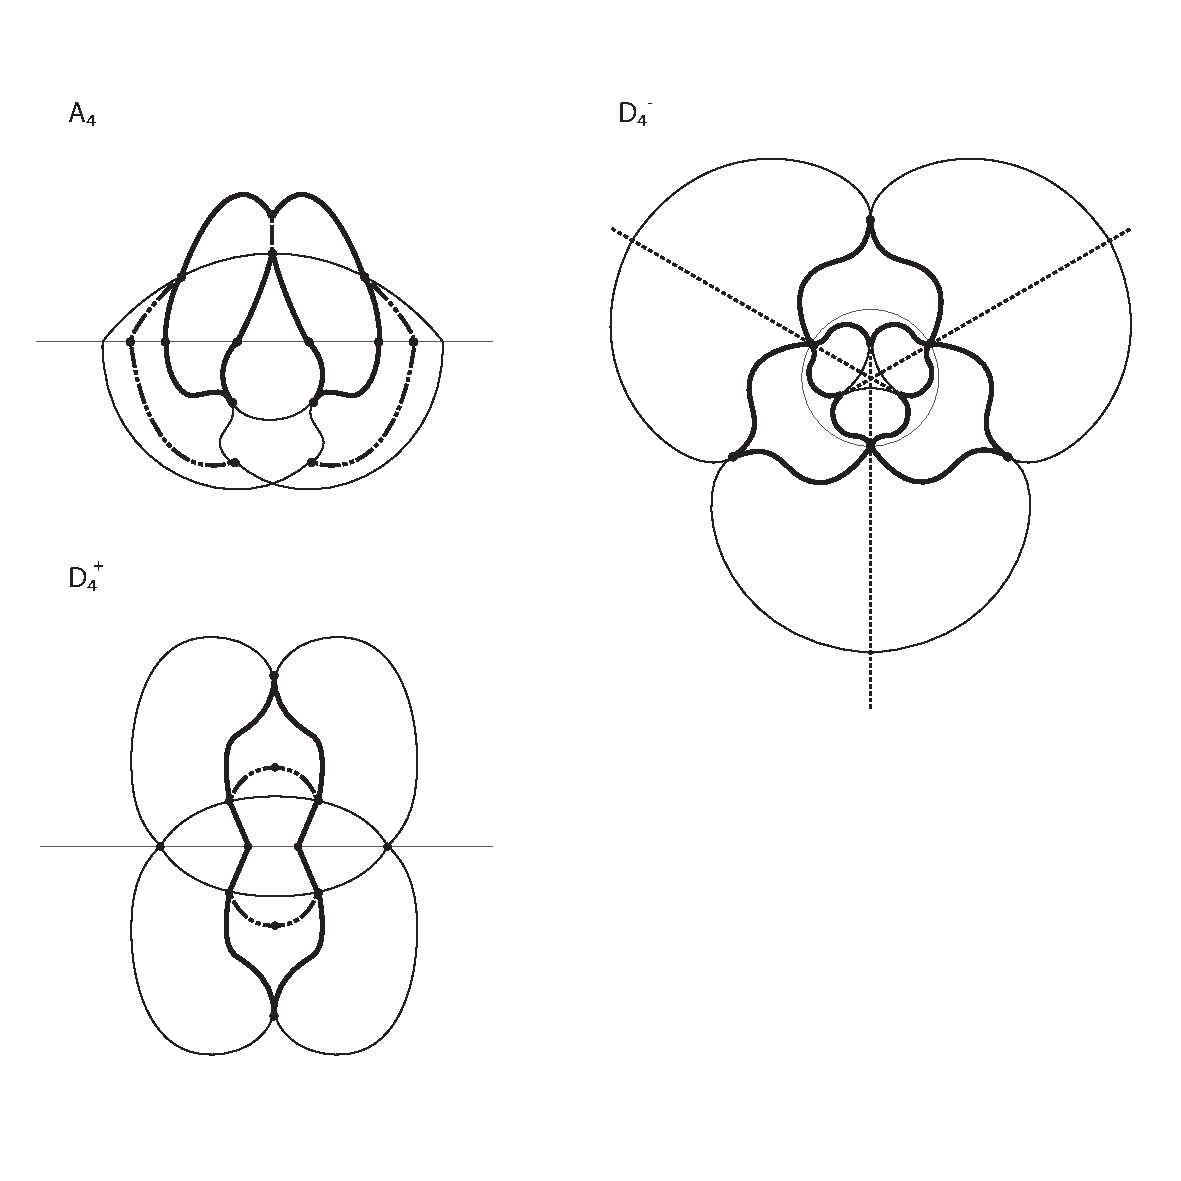
\includegraphics[width=0.9\linewidth]{Image-1-converted-to.pdf}}
		\caption{Топологическая схема каустик и множеств Стокса на $S^2$ для особенностей $A_{4}, D_{4}^-, D_{4}^+ $. Обычными линиями нарисованы каустики, жирными - расширенные множества Стокса. Для $A_4$ и $D_4^+$ пунктиром отмечены новые линии расширенного множества Стокса по сравнению с [2].  Для $ D_{4}^-$ пунктиром обозначено множество Максвелла.}\label{F7}
	\end{figure}


Пусть $f(x,\lambda):((\mathbb{C}^n,\mathbb{R}^n)\times\mathbb{R}^\mu,0)\rightarrow((\mathbb{C},\mathbb{R}),0)$ - миниверсальная деформация простой вещественной особенности, записанная в нормальной форме (см.[5]).


\begin{definition}
	Комплексное множество Стокса~--- это замыкание множества таких параметров деформации $\lambda$,
	при которых соответствующая функция $f_\lambda$ имеет комплексные (с ненулевой мнимой частью)
	критические точки (не исключено, что ещё имеет и вещественные)
	и выполняется условие на вещественные части критических значений:
	$$\mathop{\text{Re}}f_\lambda(x_i)=\mathop{\text{Re}}f_\lambda(x_j);  i\neq j,$$
	где $x_i,x_j\in\mathbb{C}^n$~--- критические точки из разных сопряжённых пар.
\end{definition}

\begin{definition}
	Смешанное множество Стокса - это замыкание множества таких параметров деформации $\lambda$,
	при которых $f_\lambda$ имеет как вещественные, так и комплексные (с ненулевой мнимой частью) критические точки,
	и выполняется условие на критические значения: $$f_\lambda(x_i)=\mathop{\text{Re}}f_\lambda(x_j); \text{где} x_i\in\mathbb{R}^n, x_j\in\mathbb{C}^n.$$
\end{definition}

\begin{definition}\
	Расширенным множеством Стокса мы будем называть объединение комплексного и смешанного множеств Стокса.
\end{definition}


\textbf{Особенность $A^4.$} Изучалась усечённая миниверсальная деформация $x^5$ в виде

$$
	f(x;a,b,c)=\dfrac{x^5}{5}+a\dfrac{x^3}{3}+b\dfrac{x^2}{2}+cx:\mathbb{C}\times\mathbb{R}^3\rightarrow\mathbb{C}.
$$

На рисунке 1 мы видим топологическую картинку стереографической проекции из точки $(0,0,1)$ в пространстве $\mathbb{R}^3=(a,b,c)$ объединения каустики и расширенного множества Стокса для $A_4$ на единичной сфере вокруг нуля в $\mathbb{R}^3.$ Горизонтальная прямая на рисунке является проекцией сечения сферы плоскостью $a=0.$ На ней мы видим 6 точек, в которых сливаются линии смешанного множества Стокса, и две точки слияния линий каустики. Далее, выше этой прямой (проекция полусферы, отвечающей условию $a>0$) мы наблюдаем, как три пары линий смешанного множества Стокса на $S^2$ сливаются в три точки на каустике, потом из этих точек выходят три линии комплексного множества Стокса, сливаясь затем в одну точку. Ниже прямой (проекция полусферы, отвечающей условию $a<0$) мы видим, как три пары линий смешанного множества Стокса подходят к каустике.

\textbf{Особенность $D_{4}^-$.}

Изучалась усечённая миниверсальная деформация особенности $x^3-xy^2$ в виде $$f(x,y;a,b,c)=x^3-3xy^2-c(x^2+y^2)-ax-by:\mathbb{C}^2\times\mathbb{R}^3\rightarrow\mathbb{C}.$$

 На рисунке 1 мы видим топологическую картинку стереографической проекции из точки $(0,0,1)$ в пространстве $\mathbb{R}^3=(a,b,c)$ объединения каустики и расширенного множества Стокса для $D_4^-$ на единичной сфере $S^2.$ Окружность на рисунке соответствует проекции $S^2\cap\{c=0\}.$ На ней мы видим три точки, в каждой из которых сливаются по две пары линий смешанного множества Стокса, пришедших из соседних углов каустики. Комплексное множество Стокса здесь пусто.

\textbf{Особенность $D_{4}^+$.}

	Изучалась усечённая миниверсальная деформация особенности $x^3+xy^2$ в виде $$f(x,y;a,b,c)=x^3+3xy^2+c(x^2-y^2)-ax-by:\mathbb{C}^2\times\mathbb{R}^3\rightarrow\mathbb{C}.$$ На рисунке 1 мы видим топологическую картинку стереографической проекции из точки $(1,0,0)$ в пространстве $\mathbb{R}^3=(a,b,c)$ объединения каустики и расширенного множества Стокса для $D_4^+$ на единичной сфере $S^2.$ Горизонтальная прямая на рисунке соответствует проекции $S^2\cap\{c=0\}$. Она же является осью симметрии. На ней мы видим две точки, в которых сливаются комплексные линии Стокса и две точки слияния линий каустики. Пара симметричных криволинейных треугольников соответствует проекции смешанного множества Стокса.



\begin{center}
	\textbf{Цитированная литература:}
\end{center}
\par
1. М. В. Федорюк Метод перевала, 1977

\selectlanguage{english}

2. M. V. Berry and C. J. Howls Stokes surfaces of diffraction catastrophes with codimension three // Nonlinearity 3 (1990) 281-291

3. Lando S. K. Geometry of Stokes sets for families of functions of one
variable // Journal of Mathematical Sciences. 1997. Vol. 83

4. Wright, Francis J. Wavefield singularities : a caustic tale of dislocation and catastrophe. A dissertation submitted to the University of Bristol
in candidature for the degree of Doctor of Philosophy, 1977

\selectlanguage{russian}

5. В. А. Васильев Ветвящиеся интегралы, 2000
